%%%%
\documentclass[10pt,answers]{exam}
\usepackage{times}
\usepackage{enumerate}
\usepackage{enumitem}
\usepackage{mathtools}
\usepackage{hyperref}
\usepackage{ragged2e}
\usepackage{graphicx}
\usepackage{blindtext}
\usepackage{pgf}
\usepackage{tikz}
\usepackage{caption}
\usepackage{subcaption}
\usepackage{blkarray}
\usepackage{amsfonts}
\usetikzlibrary{arrows,automata,matrix}

%Feel free to add packages and newcommands here if you wish
   
%%%%
% IMPORTANT: YOU SHOULD INSTANTIATE THE FOLLOWING THREE COMMANDS WITH YOUR OWN DETAILS
\newcommand{\authorname}{George Theodoridis}     %%% Write your first and last name
\newcommand{\authornumber}{S5951178}  %%% Write your student number
\newcommand{\assignmentnumber}{2}  %%% Write 1, 2, 3, etc
%%%%

%%%% DO NOT MODIFY 

\pagestyle{headandfoot}
\runningheadrule
\firstpageheader{Computer Architecture (2024-2025)}{{\textbf{Assignment}~\assignmentnumber} \\ \today}{}
\runningheader{Individual solutions by \authorname~(\authornumber)}
              {}
              {Page \thepage\ of \numpages}
\firstpagefooter{}{}{}
\runningfooter{}{}{}
\newcommand{\qpoints}[1]{\hfill \textbf{(#1 points)}}
 
\begin{document}
 \boxedpoints
\begin{center}
  \fbox{\fbox{\parbox{0.97\textwidth}{\centering
  {\Large
 \authorname~(\authornumber)  }}}
 }
\end{center}

\begin{enumerate}
\item[] \textbf{INSTRUCTIONS}

\item Submission is only via Brightspace. Deadlines are strict.

\item The exercises in this assignment add up to 100 points. To calculate your grade simply divide the number of points by 10.

\item You must submit a pdf typeset in (La)TeX (no handwritten solutions) using \textbf{this} template.

\item Seeking solutions from the internet, from any external resource, or from any other person is prohibited.

\item Please note that the course lecturer reserves the right to ask the student submitting the assignment to explain the answers to any or all questions. If the student is unable to provide a satisfactory answer then that question may receive partial/no credit. 

\item Of course, university policies on plagiarism always apply. In particular, any suspected plagiarism will be reported to the Board of Examiners.
\end{enumerate}
\rule{6cm}{0.4pt}

\bigskip
\bigskip


%%% MODIFICATIONS ALLOWED FROM HERE

\begin{questions}

\question Design an FSM for a simple calculator that performs addition, subtraction, multiplication, and division based on user input. \qpoints{15}

The calculator has the following keys on its keypad:
\begin{itemize}
    \item \textbf{Digits:} 0--9
    \item \textbf{Operators:} +, -, *, /
    \item \textbf{Calculate:} =
    \item \textbf{Reset:} C
\end{itemize}

The calculator starts in an \textit{idle} state. The user enters the first number (any number of digits), followed by an operator, and then the second number. They press the \textit{Calculate} key to display the result, after which any additional key press will return the calculator to the \textit{idle} state. Pressing the \textit{Reset} key takes the calculator to the \textit{idle} state.

\textbf{Incorrect inputs:} Any incorrect input takes the calculator to the \textit{idle} state. Incorrect inputs include:
\begin{itemize}
    \item Pressing the \textit{Calculate} button before entering the second number.
    \item Entering an operator before the first number.
    \item Entering multiple operators.
\end{itemize}

\begin{solution}
    \begin{center}
		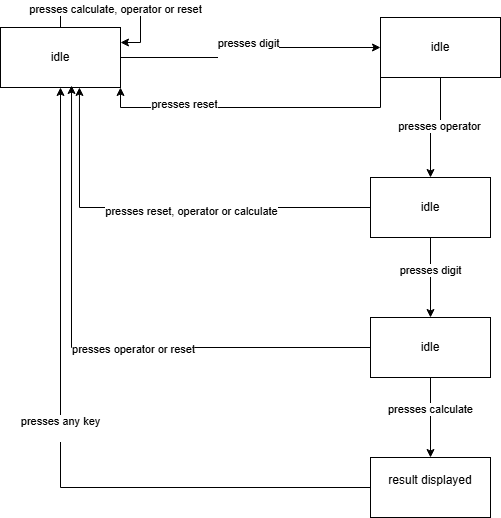
\includegraphics[width=0.6\linewidth]{ex1.png}
		\end{center}
\end{solution}

\question Assume a combinational logic circuit includes 3 inputs. Use logic gates to design a circuit to determine if the majority of the inputs are 1 or 0. \qpoints{10}

\textbf{Example:} 
\begin{itemize}
    \item \textbf{Majority 1:} 101, 110
    \item \textbf{Majority 0:} 000, 001
\end{itemize}

The following figure depicts the diagram of the circuit. The output from the majority detector is \textbf{1} if at least 2 of its inputs are 1, and \textbf{0} otherwise.

\begin{center}
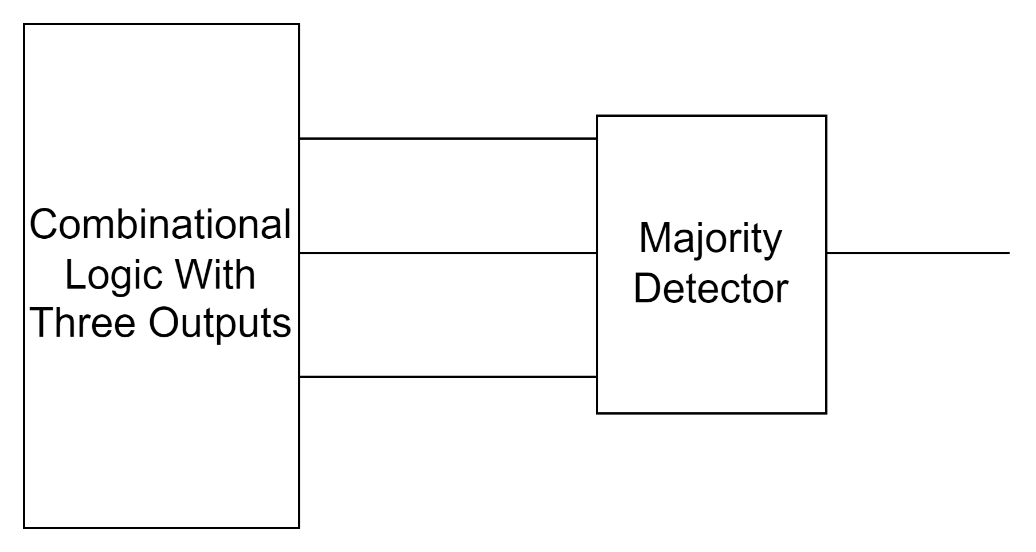
\includegraphics[width=0.6\linewidth]{images/ex2.png}
\end{center}


\begin{solution}
    \begin{center}
		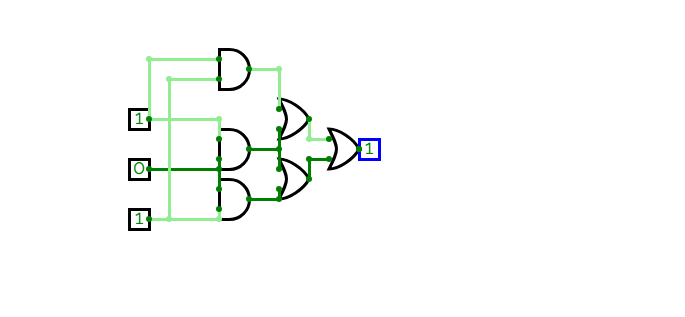
\includegraphics[width=0.6\linewidth]{ex2.png}
		\end{center}
		
\end{solution}


\question Assume that the traffic lights system is designed to include Red and Green lights. The lights are activated by the voltage input. The Selector component connects voltage input to one of the traffic lights based on the value of a counter. The 4-bit counter is used to determine which light should be active. \qpoints{15}

The system includes a 4-bit counter that determines which light should be active:
\begin{itemize}
    \item If the value of the counter is less than or equal to 5, the \textbf{Red} light will turn on.
    \item If the value of the counter is greater than 5, the \textbf{Green} light will turn on.
\end{itemize}

\textbf{Design Task:} Design the circuit for the \textit{Selector} component using logic gates. Assume the counter is provided. You only need to design the \textit{Selector} box, as shown below.

\begin{center}
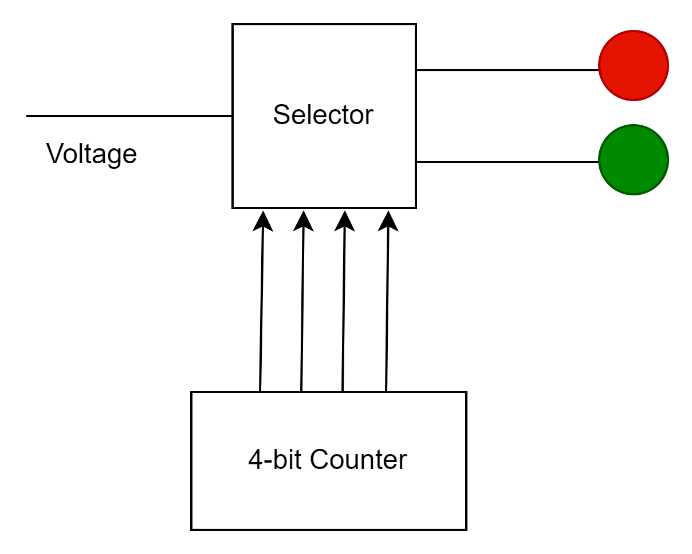
\includegraphics[width=0.6\linewidth]{images/ex3.png}
\end{center}

\begin{solution}
    \begin{center}
		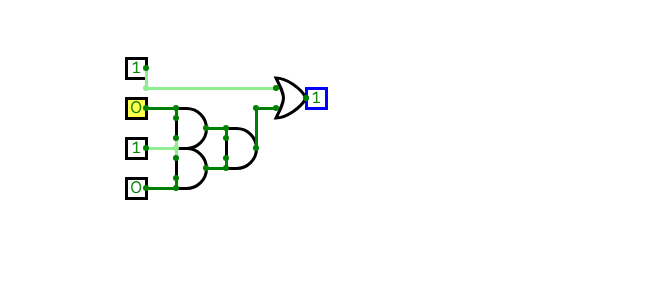
\includegraphics[width=0.6\linewidth]{ex3.png}
		1 is green 0 is red
		\end{center}
\end{solution}


\question The addressability of the memory system of a computer is two bytes. You need 18 bits to access a location in memory. What is the total size of the memory in Bytes? \qpoints{10}

\begin{solution}
    $2^{18} = 262,144$
\end{solution}


\question Design a circuit to multiply two 2-bit binary numbers. You may use logic gates or adders. \qpoints{15}

\begin{solution}
    \begin{center}
		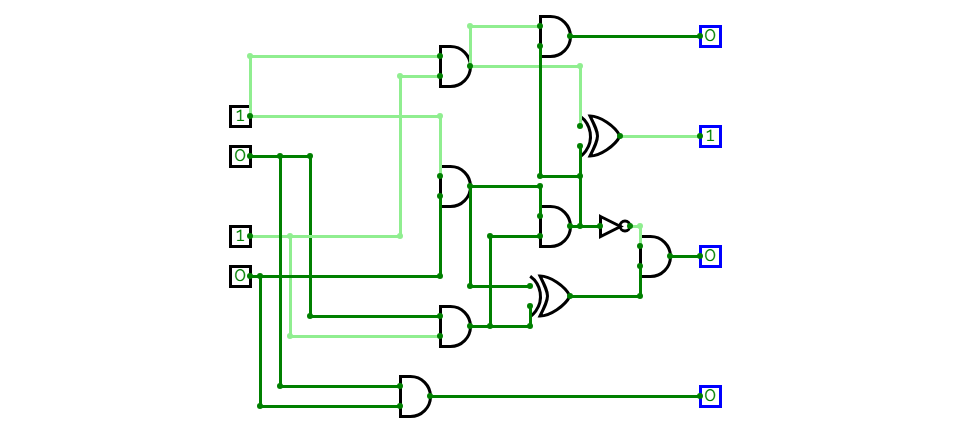
\includegraphics[width=0.6\linewidth]{ex5.png}
	\end{center}
\end{solution}



\question In the following shift register, select bits of the multiplexers determine the operation. 

The register can: \qpoints{10}

\begin{itemize}
    \item Preserve the current value.
    \item Shift left with serial input from the least significant bit.
    \item Shift right with serial input from the most significant bit.
    \item Accept parallel input.
\end{itemize}

\textbf{Design Task:} Modify the circuit to perform circular shifts instead of serial input shifts. 
\begin{itemize}
    \item In a \textbf{left circular shift}, the most significant bit is placed at the least significant bit position.
    \item In a \textbf{right circular shift}, the least significant bit is placed at the most significant bit position.
\end{itemize}

\textbf{Examples:}
\begin{itemize}
    \item Current value: 0011
    \item After left circular shift: 0110
    \item After right circular shift: 1001
\end{itemize}

\begin{center}
    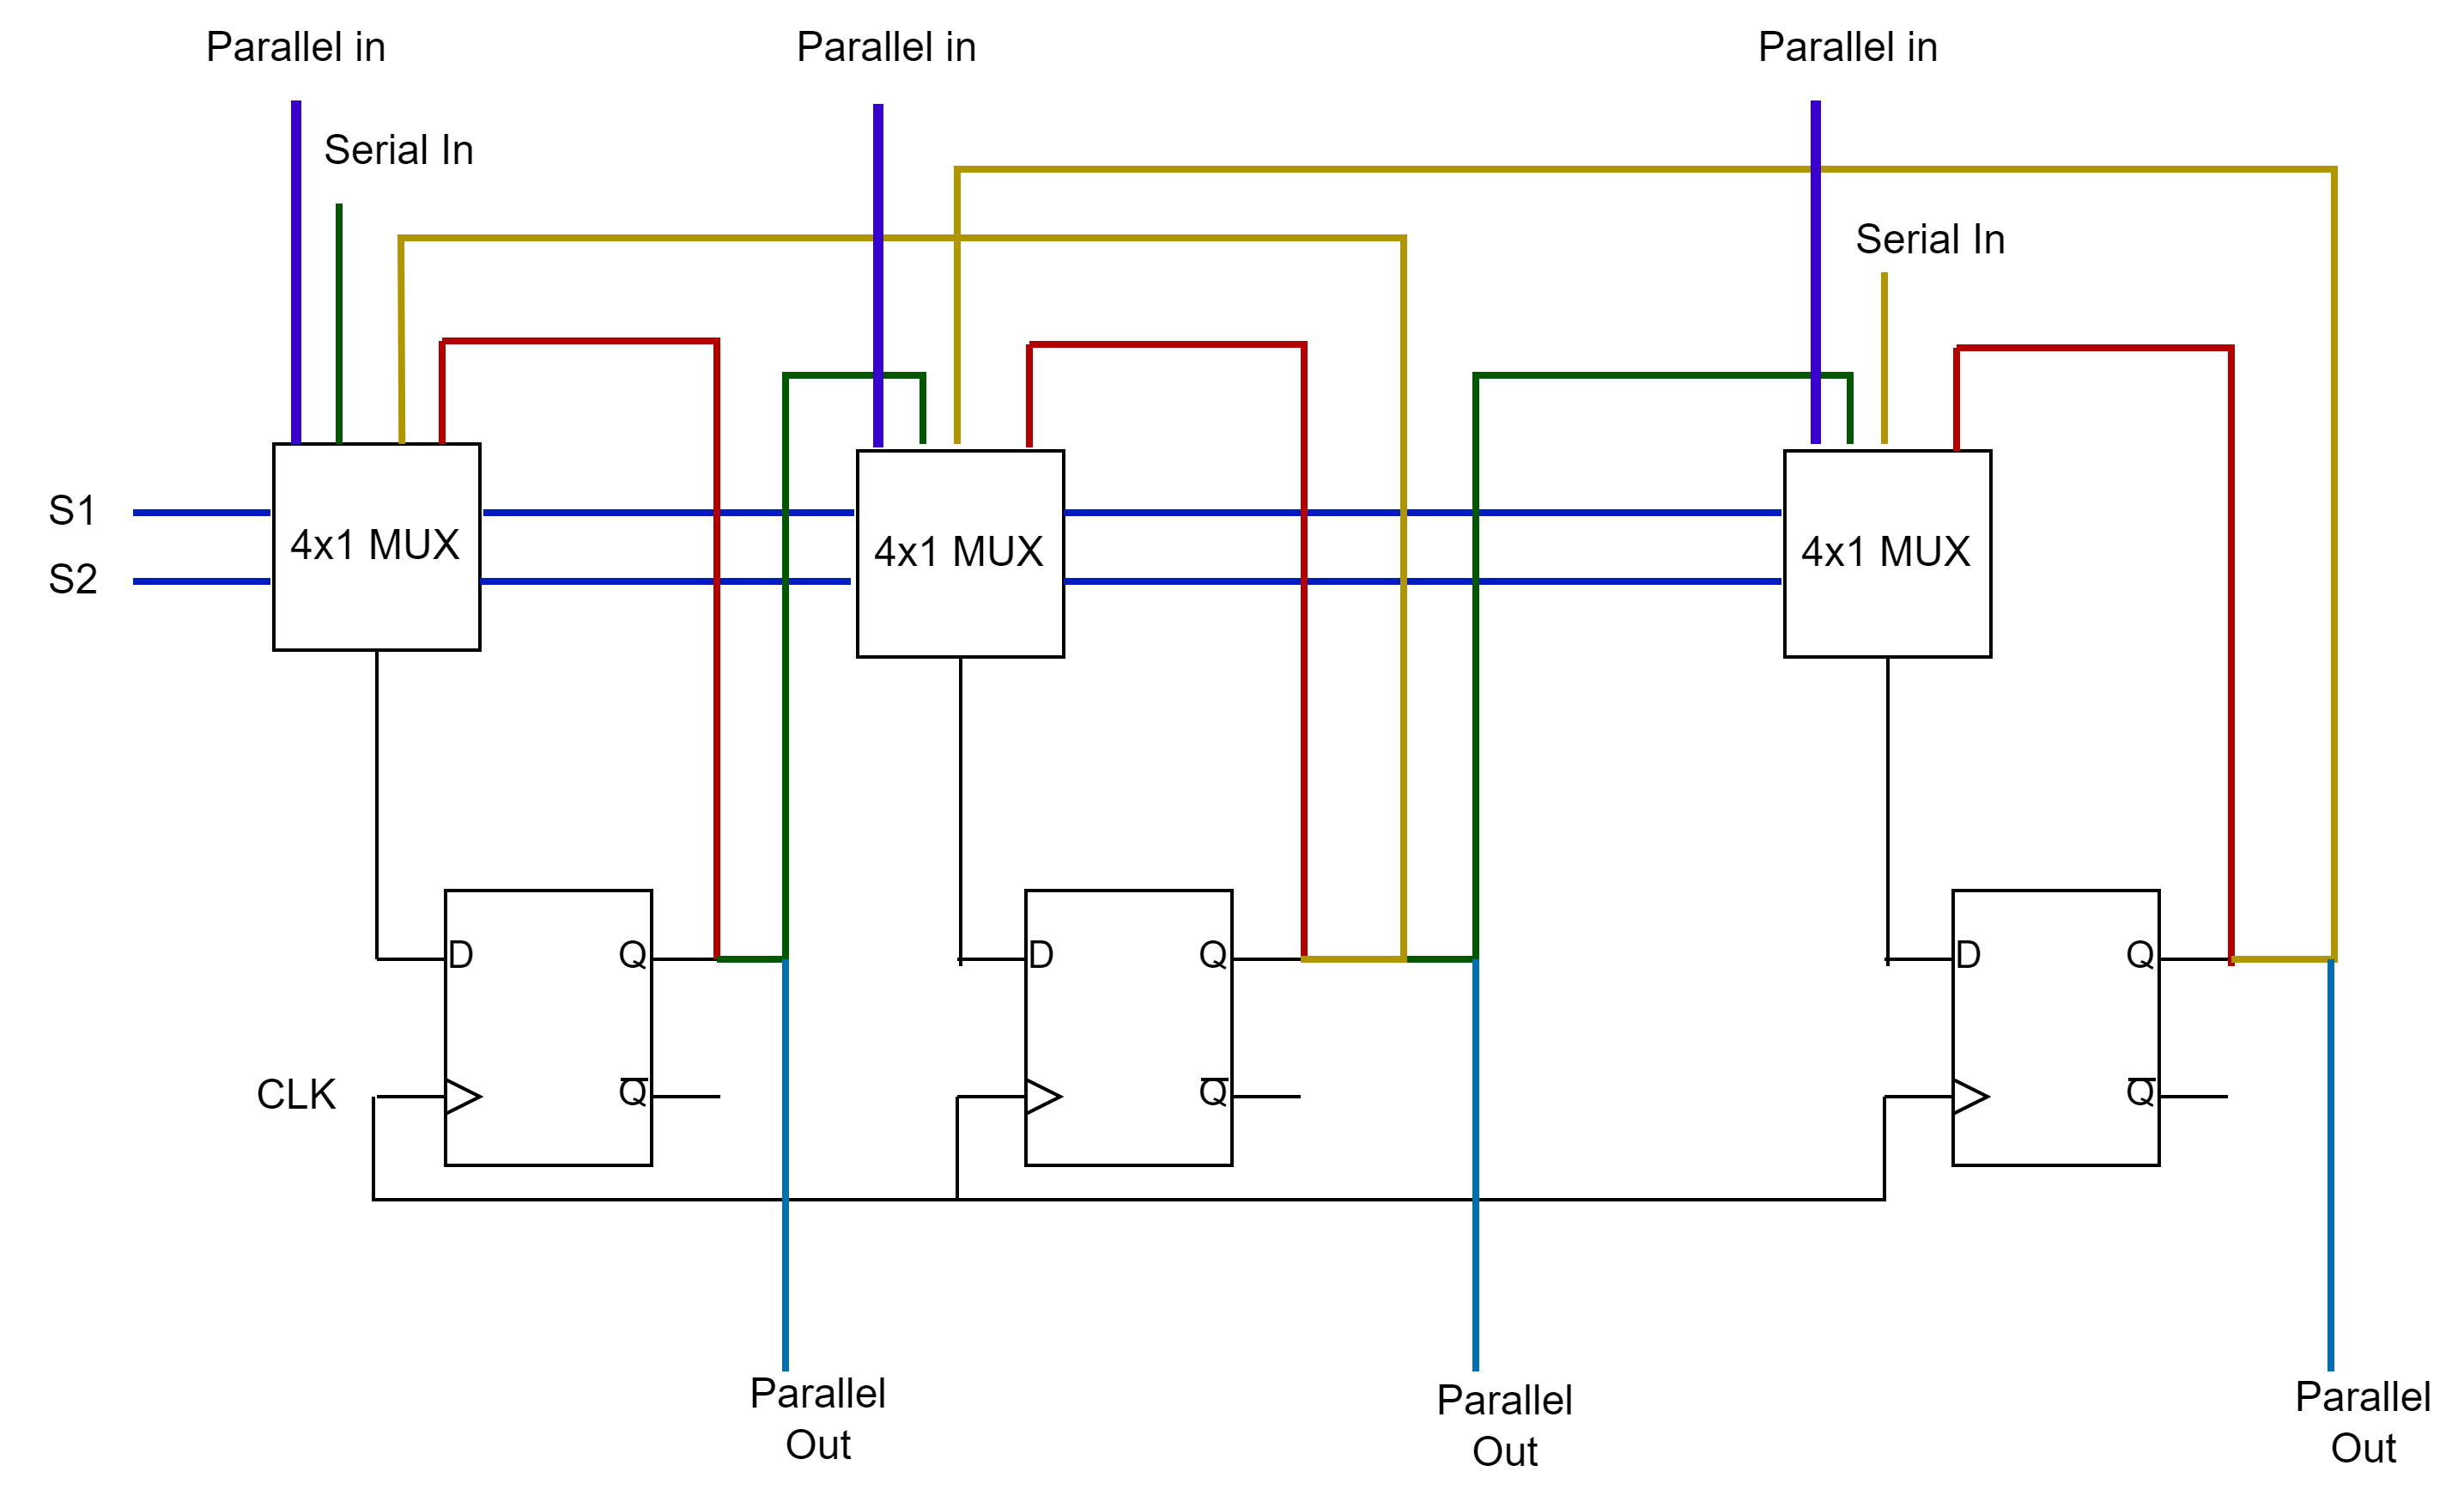
\includegraphics[width=0.75\linewidth]{images/ex6.png}
\end{center}

\begin{solution}
    \begin{center}
		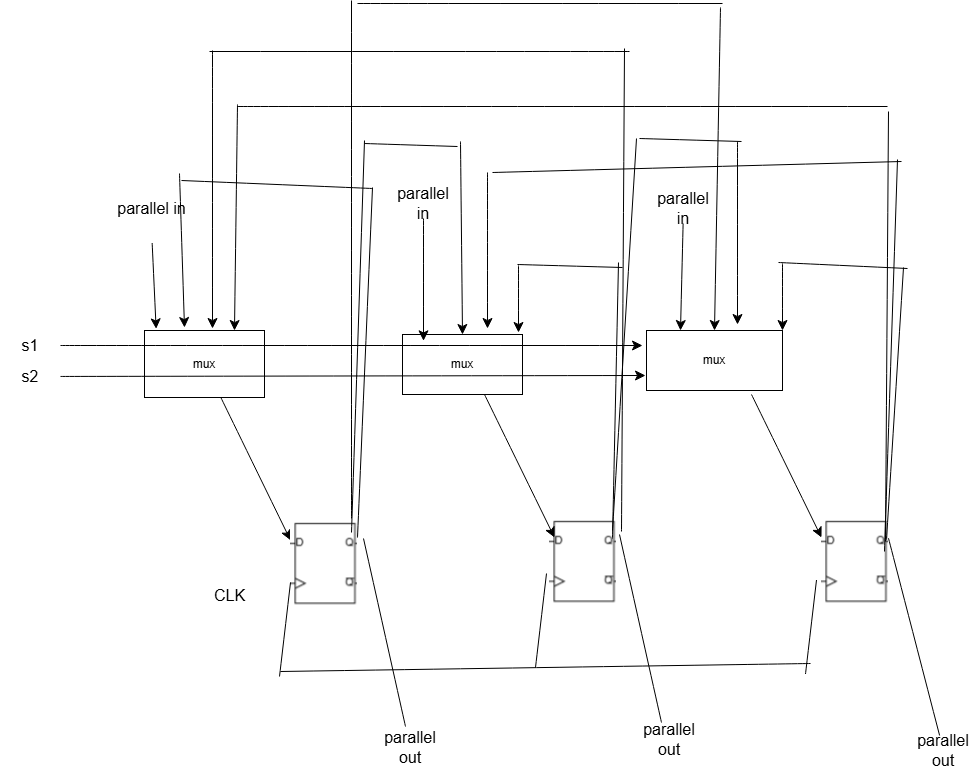
\includegraphics[width=0.6\linewidth]{ex6.png}
		\end{center}
\end{solution}


\question The following figure depicts a combinational logic circuit of a 2-to-4 decoder (two inputs $A_1$ and $A_0$ and $2^2$ outputs: $F_3, F_2, F_1, F_0$) with an enable input signal $E$. \qpoints{10}

\begin{center}
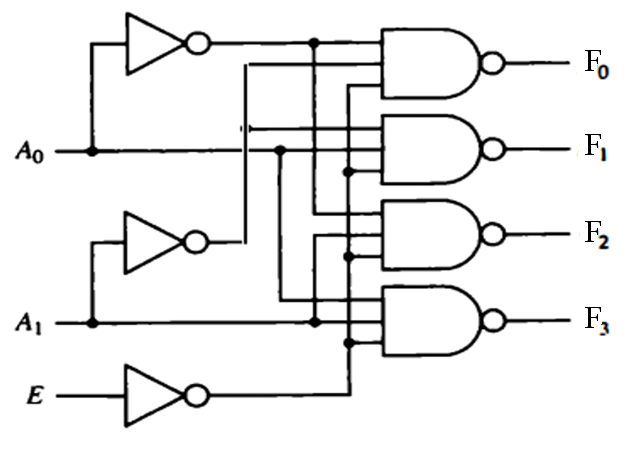
\includegraphics[width=0.5\linewidth]{images/ex7.png}
\end{center}

\begin{enumerate}[label=\alph*)]
    \item Fill all of the missing values in the following truth table and provide the steps you followed to obtain your answers. Please note that symbol $X$ in the table can represent both 0 or 1 (the so-called “don’t care”).
\begin{solution}
    \begin{center}
        \begin{tabular}{|c|c|c|c|c|c|c|c|}
        \hline
        $E$ & $A_1$ & $A_0$ & $F_3$ & $F_2$ & $F_1$ & $F_0$ \\ \hline
        1   & X     & X     & 1      & 1      & 1       & 1      \\ \hline
        0   & 0     & 0     & 1      & 1      & 1      & 0      \\ \hline
        0   & 0     & 1     & 1      & 1      & 0      & 1      \\ \hline
        0   & 1     & 0     &  1     & 0      & 1      & 1      \\ \hline
        0   & 1     & 1     & 0      & 1      & 1      & 1      \\ \hline

        \end{tabular}

		\section*{Case 1}
\begin{itemize}
    \item $E = 1$, $A_1 = X$, $A_0 = X$
    \item When $E = 1$, $\overline{E} = 0$, disabling all outputs.
    \item All $F_i = 1$ (don’t care about $A_1$ and $A_0$).
\end{itemize}

\section*{Case 2}
\begin{itemize}
    \item $E = 0$, $A_1 = 0$, $A_0 = 0$
    \item $\overline{E} = 1$, circuit enabled.
    \item Decoder activates $F_0 = 0$, leaving $F_1, F_2, F_3 = 1$.
\end{itemize}

\section*{Case 3}
\begin{itemize}
    \item $E = 0$, $A_1 = 0$, $A_0 = 1$
    \item $\overline{E} = 1$, circuit enabled.
    \item Decoder activates $F_1 = 0$, leaving $F_0, F_2, F_3 = 1$.
\end{itemize}

\section*{Case 4}
\begin{itemize}
    \item $E = 0$, $A_1 = 1$, $A_0 = 0$
    \item $\overline{E} = 1$, circuit enabled.
    \item Decoder activates $F_2 = 0$, leaving $F_0, F_1, F_3 = 1$.
\end{itemize}

\section*{Case 5}
\begin{itemize}
    \item $E = 0$, $A_1 = 1$, $A_0 = 1$
    \item $\overline{E} = 1$, circuit enabled.
    \item Decoder activates $F_3 = 0$, leaving $F_0, F_1, F_2 = 1$.
\end{itemize}
    \end{center}
\end{solution}

    \item How many 2-to-4 decoders are needed to design a 4-to-16 decoder? Explain your answer.
\end{enumerate}

\begin{solution}
    5 decoders: 1 main 2-to-4 decoder which will enable the first 2 bits of the input, and 4 2-to-4 decoders which each will connect to each output of the first decoder and they will respresent the remaining 2 bits.
\end{solution}


\question Design a logic unit capable of performing \textbf{AND}, \textbf{OR}, \textbf{XOR}, \textbf{NAND}, \textbf{NOR}, and \textbf{XNOR} operations on two 1-bit inputs. 

Use a 4x1 multiplexer to select the desired operation and a 3x8 decoder to generate control signals. \qpoints{15}

The desired operation is given as a 3-bit value, as shown below:

\begin{center}
    \begin{tabular}{|c|c|}
        \hline
        \textbf{Operation} & \textbf{Code} \\ \hline
        AND & 000 \\ \hline
        OR & 001 \\ \hline
        XOR & 010 \\ \hline
        NAND & 011 \\ \hline
        NOR & 100 \\ \hline
        XNOR & 101 \\ \hline
    \end{tabular}
\end{center}

\begin{solution}
    \begin{center}
		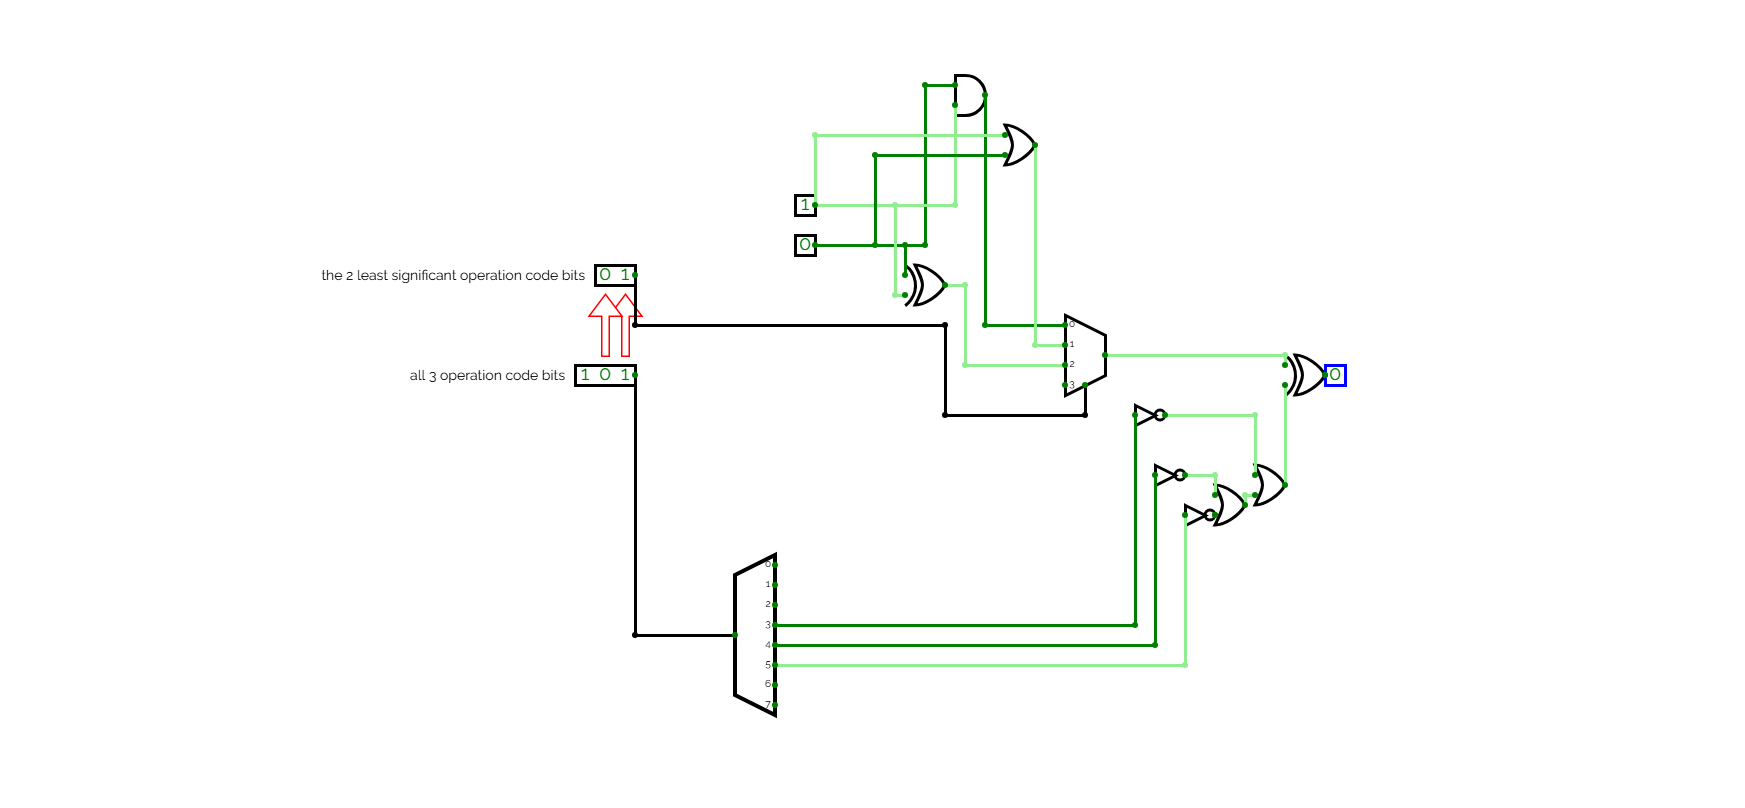
\includegraphics[width=0.5\linewidth]{ex8.png}
		\end{center}
\end{solution}


\end{questions}
\end{document}
